\documentclass[convert={density=300,size=1080x800,outext=.png}]{standalone}
\usepackage{pgfplots}
\usepackage{tikz}

\usetikzlibrary{calc}
\usetikzlibrary{patterns,angles,quotes}

\usetikzlibrary{shapes.misc}

% From http://tex.stackexchange.com/questions/123760/draw-crosses-in-tikz
\tikzset{cross/.style={cross out, draw=black, fill=none, minimum size=2*(#1-\pgflinewidth), inner sep=0pt, outer sep=0pt}, cross/.default={2pt}}

\begin{document}
	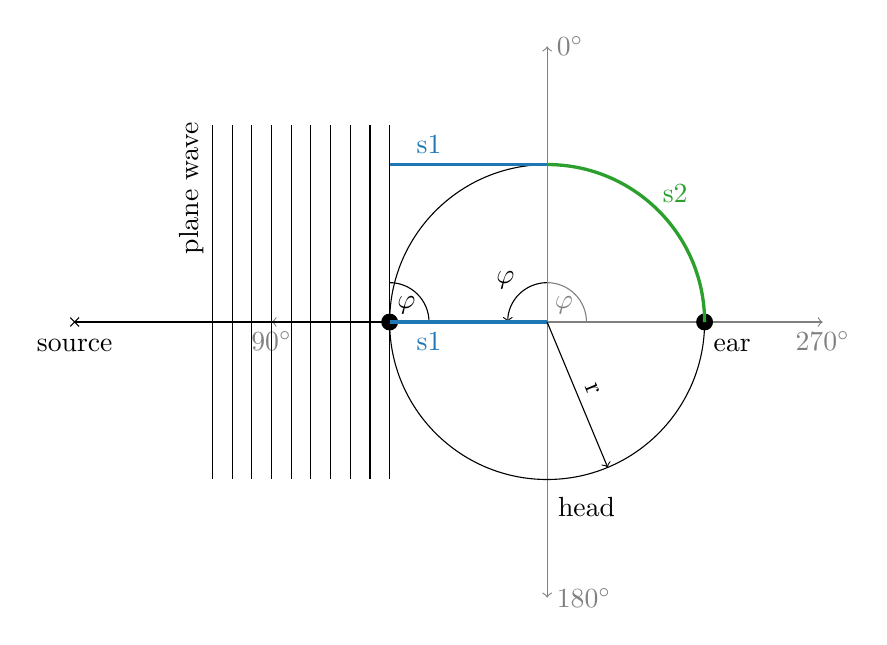
\begin{tikzpicture} 
	
	\definecolor{color0}{rgb}{0.12156862745098,0.466666666666667,0.705882352941177}
	\definecolor{color1}{rgb}{1,0.498039215686275,0.0549019607843137}
	\definecolor{color2}{rgb}{0.172549019607843,0.627450980392157,0.172549019607843}
	\definecolor{color3}{rgb}{0.83921568627451,0.152941176470588,0.156862745098039}
	\definecolor{color4}{rgb}{0.580392156862745,0.403921568627451,0.741176470588235}
	\definecolor{color5}{rgb}{0.549019607843137,0.337254901960784,0.294117647058824}
	
	% coordinate System
	\draw [<->, gray] (-3.5,0) -- (3.5,0);
	\draw [<->, gray] (0, -3.5) -- (0, 3.5);
	\node at (-3.5,0) [left, below, gray] {$90^{\circ}$};
	\node at (3.5,0) [right, below, gray] {$270^{\circ}$};
	\node at (0,-3.5) [right, gray] {$180^{\circ}$};
	\node at (0,3.5) [right, gray] {$0^{\circ}$};
	
	% define points
	\coordinate (R) at (0,0); %receiver

	% coordinate for source
	\def \Sx {-6};
	\def \Sy {0};	
	\coordinate (S) at (\Sx, \Sy); %source
	


	%triangle coordinats
	\coordinate (A) at (-2, 0);
	\coordinate (B) at ($(R)!(A)!(S)$);
	
	%corrdinate for angle phi
	\coordinate (Y) at (0,3.5);
	\coordinate (X) at (3.5,0);
	
	% big triangle
%	\def \mt {-\Sx / \Sy};
	\coordinate (C) at (0,2);
	
	% coordinate for radius
	\coordinate (C2) at (0.77, {-0.77*(6/2.5)});
	
	
	
	% draw source
	\draw (S) node[cross] {};
	\node at (S) [below, yshift = -1mm]{source};
	
	% draw head
	\draw (R) circle (2cm);
	\node at ($(R)-(0cm, 2cm)$) [below, yshift = -1mm, xshift = 0.5cm] {head};
	\filldraw (A) circle (1mm);
	\filldraw ($(R)+(2cm,0cm)$) circle (1mm);
	\node at ($(R)+(2cm,0cm)$) [yshift = -0.3cm, xshift = 0.35cm]{ear};
	
	% line RS
	\draw (S) -- (R);
	
	% plane wave

	\def \m {\Sy / \Sx}; % slope
	\def \Ax {-2};
	\def \Ay {0};
	\def \n {\Ay - (\Ax * \m)} 
	
	\foreach \x in {-4.25, -4.0, -3.75, -3.5, -3.25, -3.0, -2.75, -2.5, -2.25}
		\draw [shorten >=-2cm, shorten <=-2.5cm] ($(R)!({\x},{(\x*\m)+\n})!(S)$) -- ({\x},{(\x*\m)+\n});
	

	
	% plane wave
	
%	\def \PWx {-4};
%	\def \PWy {4};
%	\coordinate (PW) at (\PWx, \PWy);
%	\def \n {\PWy - (\PWx * \m)};
%	\draw [shorten <=-2cm] ($(R)!(PW)!(S)$) -- (PW);
%	\foreach \x in {-3.75, -3.5, -3.25, -3.0, -2.75, -2.5, -2.25}
%		\draw [shorten <=-2cm] ($(R)!({\x},{(\x*\m)+\n})!(S)$) -- ({\x},{(\x*\m)+\n});
	
	% angle 
	\pic [draw, ->, "$\varphi$", angle eccentricity=1.5] {angle = Y--R--S};
	\pic [draw, "$\varphi$"] {angle = R--A--B};
	\pic [gray, draw, "$\varphi$"] {angle = X--R--C};
	
	% triangle
	\draw [shorten >=-2.cm, shorten <=-2.5cm](A) -- node[below,sloped,  yshift = 2.8cm, xshift = 1.7cm] {plane wave} (B);	
	\draw [shorten <=-3.2cm,shorten >=-1.cm, dashed, gray](R) -- (C);
	
	% s1 and s2
	\draw [color0, very thick] (C) -- node [above, sloped, near end] {s1}  ($(A)!(C)!(B)$);
	\draw [color0, very thick] (B) -- node [below, sloped, near start] {s1}  (R);
	\draw pic[draw = color2, "s2", text =color2, angle eccentricity=1.15, angle radius=20mm, line width = 1.2]{angle=X--R--C} ;
	
	%radius
	\draw [->] (R) -- node [right, sloped, midway, above]{r}(C2);
	
	\end{tikzpicture}
\end{document}